\documentclass{beamer}    % 14pt je nenujen
\usepackage[T1]{fontenc}
\usepackage[utf8]{inputenc}
\usepackage[slovene]{babel}
\usepackage{pgfpages}           % privat zapiski
\usepackage{amsfonts}
\usepackage{amsmath,amsthm}     % pravilen izpis v "math mode"
%\usepackage{hyperref}
\usepackage{graphicx}           % za slike
\usepackage{tikz}
\usepackage{multicol}
\usepackage{ulem}
\usepackage{bibentry}

%\hypersetup{hidelinks}

\setbeamertemplate{theorems}[ams style]             % numbered da brez bold 

\setbeameroption{hide notes}                        % samo prosojnice
%\setbeameroption{show only notes}                   % samo zapiski
%\setbeameroption{show notes on second screen=right}  % oboje

\usepackage{palatino}
\usefonttheme{serif}

%\usecolortheme{beetle} %ali beetle morda ali seagull 

\setbeamertemplate{navigation symbols}{} % izklop navigacije
\setbeamertemplate{footline}[frame number]{} % oštevilčenje
\setbeamertemplate{note page}{\pagecolor{yellow!5}\insertnote}

\newtheorem{izrek}{Izrek}
\newtheorem{trditev}[izrek]{Trditev}
\newtheorem{posledica}[izrek]{Posledica}
\newtheorem{definicija}[izrek]{Definicija}
\newtheorem{naloga}[izrek]{Naloga}
\newtheorem{resitev}[izrek]{Naloga}

\author{Tim Kalan \\ \medskip
        \footnotesize Mentor: doc.~dr. Tilen Marc}
% \author{Tim Kalan}
% \institute[FMF]{Fakulteta za matematiko in fiziko}
% \title{
%     Kako se skupina podpiše? \\ 
%     \large (angl. \textit{How can a group sign?})}
\title{Kako se skupina podpiše?}
\date{27. maj 2024} 



\begin{document}

\begin{frame}
    \titlepage
\end{frame}

\begin{frame}
    \frametitle{Zakaj potrebujemo podpise?}
    \begin{itemize}
        \item Mislim, da si lahko predstavljate ... 
        \item Avtentikacija, integriteta
        \item Bančništvo, e-pošta, \texttt{ssh}, ...
    \end{itemize}
\end{frame}

\begin{frame}
    \frametitle{Kaj je podpis?}
    \begin{multicols*}{2}
        \textbf{Ročni podpis}
        \begin{itemize}
            \item Vsakič (približno) enak
            \item Enostavno ponarediti
            \item Težko (zares) preveriti
        \end{itemize}
        \columnbreak

        \textbf{Digitalni podpis}
        \begin{itemize}
            \item Vsakič unikaten
            \item Težko ponarediti
            \item Enostavno preveriti
        \end{itemize}
    \end{multicols*}
\end{frame}

\begin{frame}
    \frametitle{Kriptografija javnega ključa 1}
    \begin{figure}
        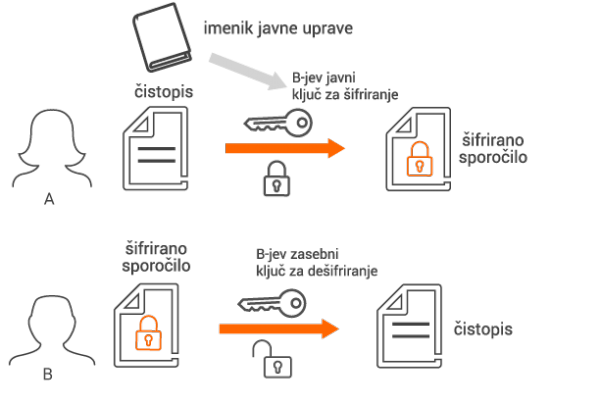
\includegraphics[width=\textwidth]{images/enkripcija.png}
    \end{figure}
\end{frame}

\begin{frame}
    \frametitle{Kriptografija javnega ključa 2}
    \begin{figure}
        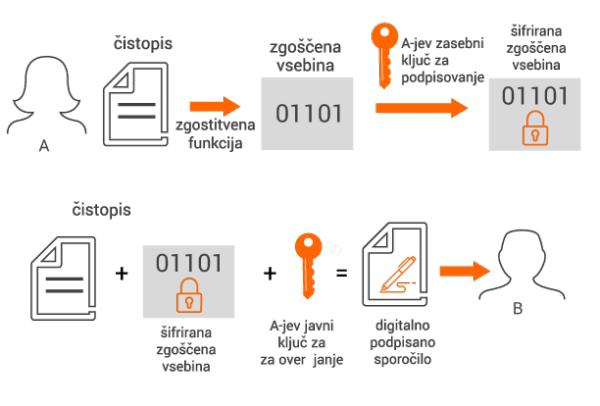
\includegraphics[width=\textwidth]{images/podpisovanje.png}
    \end{figure}
\end{frame}

\begin{frame}
    \frametitle{Zgostitvene funkcije}
\end{frame}

\begin{frame}
    \frametitle{Primer digitalnega podpisa: RSA}
    Odličen primer za spoznavanje osnovnih konceptov:
    \vspace{1cm}
    \begin{itemize}
        \item Generiranje ključev
        \item Podpisovanje
        \item Preverjanje 
    \end{itemize}
\end{frame}

\begin{frame}
    \frametitle{RSA: Generiranje ključev}
    \begin{itemize}
        \item Izberemo dve \alert{veliki} praštevili $p$ in $q$ (kako?)
        \item Izračunamo $n = pq$ in $\phi(n) = (p-1)(q-1)$
        \item Izberemo $e$ tako, da je $1 < e < \phi(n)$ in $\gcd(e, \phi(n)) = 1$
        \item Izračunamo $d$ tako, da je $ed \equiv 1 \pmod{\phi(n)}$
    \end{itemize}
    \begin{multicols*}{2}
        \textbf{Javni ključ}: $(n, e)$
        \columnbreak

        \textbf{Zasebni ključ}: $d$
    \end{multicols*}
\end{frame}

\begin{frame}
    \frametitle{RSA: Podpisovanje in preverjanje}
    \begin{itemize}
        \item Sporočilo $m$ podpišemo tako, da izračunamo $s = m^d \bmod n$
        \item Podpis je par $(m, s)$
    \end{itemize}
    
    \vspace{1cm}
    \begin{itemize}
        \item Preverimo tako, da izračunamo $m' = s^e \bmod n$
        \item Podpis je pravilen, če je $m' = m$
    \end{itemize}
\end{frame}

\begin{frame}
    \frametitle{RSA: Primer}
\end{frame}

\begin{frame}
    \frametitle{Kako se skupina podpiše?}
    \begin{itemize}
        \item \textbf{Prilagodljivost} (angl. \textit{flexibility})
        \item \textbf{Odgovornost} (angl. \textit{accountability})
    \end{itemize}
    \vspace{1cm}
    \textbf{Skupina}: 
    \begin{align*}
        G &= P_1, P_2, \dots, P_L \\
        S &\subseteq G
    \end{align*}
\end{frame}

\begin{frame}
    \frametitle{Skupinski podpisi (angl. \textit{group signatures})}
    \begin{itemize}
        \item Anonimen podpis v imenu skupine
        \item Ni prilagodljivosti
        \item Delna odgovornost (vodja skupine)
        \item Primer: 
    \end{itemize}
\end{frame}

\begin{frame}
    \frametitle{Mejni podpisi (angl. \textit{threshold signatures})}
    \begin{itemize}
        \item $t$-od-$n$ shema
        \item Zmerna prilagodljivost
        \item Ni odgovornosti
        \item Primer: 
    \end{itemize}
\end{frame}

\begin{frame}
    \frametitle{Naivna ideja}
    \begin{itemize}
        \item Želimo si prilagodljivost in odgovornost
        \item Vsak član $S$ podpiše $(M, S) \rightarrow \sigma_i$
        \item Kot na papirju
        \item Primer:
    \end{itemize}
    \vspace{1cm}
    \pause
    Težava?
        $\sigma_1, \sigma_2, \sigma_3, \sigma_4, \sigma_5, \sigma_6,
        \sigma_7,  \sigma_8, \sigma_9, \sigma_{10}, \sigma_{11}, \sigma_{12}, 
        \sigma_{13}, \sigma_{14}, \sigma_{15}, \dots$
\end{frame}

\begin{frame}
    \frametitle{Skupni podpisi (angl. \textit{multisignatures})}
    \begin{itemize}
        \item Skupina vrne samo en podpis
        \item Prilagodljivost in odgovornost
        \item Naivna ideja + učinkovitost
        \item Primer:
    \end{itemize}
\end{frame}

\begin{frame}
    \frametitle{Schnorrov podpis}
    \textbf{Generiranje ključa} \\
    \begin{itemize}
        \item 
    \end{itemize}
    \textbf{Podpisovanje} \\
    \begin{itemize}
        \item 
    \end{itemize}
    \textbf{Verifikacija}
    \begin{itemize}
        \item 
    \end{itemize}
\end{frame}

\begin{frame}
    \frametitle{Varnost}
\end{frame}

\end{document}